\chapter{Giản đồ Penrose và sự hình thành của một lỗ đen thực}

Biểu diễn Kruskal cho một mô tả thanh nhã về lân cận của chân trời Schwarzschild, nhưng một lỗ đen thực không phải là vĩnh cửu: nó hình thành khi vật chất sụp đổ. Những phần nào của biểu diễn mở rộng còn tồn tại qua lịch sử vật lý đó? Để trả lời câu hỏi này, ta cần một giản đồ đủ lớn để chứa trọn một không-thời gian và đủ chặt chẽ để bảo toàn chuyển động của ánh sáng. Trước hết ta sẽ compact hóa không-thời gian phẳng, rồi compact hóa không-thời gian Schwarzschild, và cuối cùng khâu các mảnh thích hợp lại với nhau qua một vỏ bức xạ rơi vào.

\section{Gần chân trời: ôn lại Kruskal và bốn góc phần tư}

Ta bắt đầu đúng ngay chỗ bài giảng trước đã dừng lại. Rất gần chân trời Schwarzschild, hình học trông cục bộ như không gian phẳng. Bản thân chân trời ứng xử như một quỹ tích tọa độ cực hyperbol, cũng như các tọa độ gia tốc trong không-thời gian Minkowski thông thường. Trong bức tranh cục bộ này, ngay từ đầu ta áp đặt một quy tắc và không bao giờ nới lỏng nó: các tia sáng xuyên tâm được vẽ ở \(45^\circ\), và mọi đường thế giới kiểu thời gian đều phải dốc hơn các đường null ấy.

Các tọa độ trong phần ôn lại này tốt nhất nên được hiểu là thời gian và không gian theo cách một quan sát viên rơi vào nhìn thấy. Trong các tọa độ quán tính cục bộ đó, lân cận của chân trời trông gần như phẳng. Nhưng một quan sát viên cứ khăng khăng lơ lửng ở bán kính cố định bên ngoài lỗ đen thì không phải là quán tính. So với hệ quy chiếu của người rơi vào, người như vậy vạch nên một đường cong gia tốc. Càng lơ lửng gần chân trời thì gia tốc cần để ở ngoài càng lớn. Đó chính là nội dung vật lý của họ các đường cong bên ngoài được vẽ ở phía bên phải bảng.

\begin{figure}[htbp]
\centering
\includegraphics[width=0.72\textwidth]{lecture_08_figure_02.png}
\caption{Phác thảo trên bảng về hình học gần chân trời gồm bốn miền. Các đường cong đỏ ở miền ngoài biểu diễn một họ đường thế giới lơ lửng tại bán kính cố định.}
\lectureframe{00:02:54}
\end{figure}

\begin{figure}[htbp]
\centering
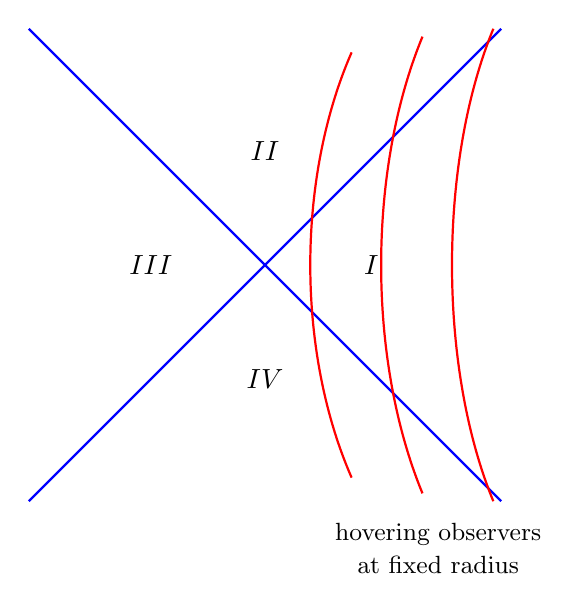
\begin{tikzpicture}[scale=1.0]
\draw[thick,blue] (-3,3) -- (3,-3);
\draw[thick,blue] (-3,-3) -- (3,3);

\draw[red,thick] (1.1,-2.7) .. controls (0.4,-1.1) and (0.4,1.1) .. (1.1,2.7);
\draw[red,thick] (2.0,-2.9) .. controls (1.3,-1.2) and (1.3,1.2) .. (2.0,2.9);
\draw[red,thick] (2.9,-3.0) .. controls (2.2,-1.3) and (2.2,1.3) .. (2.9,3.0);

\node at (1.35,0.0) {$I$};
\node at (0.0,1.45) {$II$};
\node at (-1.45,0.0) {$III$};
\node at (0.0,-1.45) {$IV$};

\node[align=center] at (2.2,-3.6) {\small hovering observers\\\small at fixed radius};
\end{tikzpicture}
\caption{Vẽ lại rõ ràng cấu trúc nhân quả kiểu Kruskal được dùng trong phần ôn lại. Miền \(I\) là miền ngoài, miền \(II\) là miền trong không thể thoát ra, còn các miền \(III\) và \(IV\) thuộc về phần mở rộng hình thức mà về sau sẽ bị loại bỏ đối với một lỗ đen thực hình thành do sụp đổ.}
\end{figure}

Chừng đó đã đủ để nói lỗ đen làm gì. Trong miền ngoài \(I\), các vật thể và tín hiệu có thể đi vào trong, nhưng chúng cũng có thể ở lại bên ngoài hoặc quay trở ra. Trái lại, trong miền \(II\), kết luận nhân quả là dứt khoát. Một khi đã ở trong miền trong thì không có đường nhân quả hướng tương lai nào quay lại miền ngoài. Muốn thoát từ miền \(II\) sang một trong hai miền bên ngoài sẽ đòi hỏi một quỹ đạo ở đâu đó thoải hơn \(45^\circ\), và vì thế nhanh hơn ánh sáng. Mọi quỹ đạo kiểu thời gian hướng tương lai được phép đều kết thúc ở kỳ dị.

Phần ôn lại mở đầu này không chỉ đơn thuần là lặp lại. Nó chuẩn bị cho chủ đề chính của chương. Biểu diễn Kruskal hữu ích, nhưng không phải toàn bộ của nó đều có ý nghĩa vật lý đối với một lỗ đen thực.

\begin{classroomqa}
\audiencequestion{Các trục của giản đồ là gì, và các đường cong đỏ là những đường thế giới vị trí cố định của ai?}
\lecturerresponse{Các trục là thời gian và không gian trong hệ tọa độ tự nhiên đối với một quan sát viên rơi tự do. Gần chân trời, quan sát viên đó nhìn thấy một không-thời gian gần như phẳng thông thường. Trái lại, các đường cong vị trí không đổi màu đỏ thuộc về những quan sát viên bị giữ đứng yên bên ngoài lỗ đen. Chúng là các đường thế giới gia tốc, với gia tốc cần thiết tăng lên khi tiến về phía chân trời.
\lecturetimestamp{00:05:58--00:06:47}}
\end{classroomqa}

\section{Vì sao phải compact hóa? Từ không-thời gian vô hạn đến một tấm bảng hữu hạn}

Bước tiếp theo mang tính phương pháp. Các hướng null trong những giản đồ này đi ra vô hạn, và bản thân thời gian cũng vậy. Vì thế ta không thể vẽ toàn bộ không-thời gian trên một tấm bảng thông thường trừ khi thay đổi tọa độ. Động cơ của giảng viên rất cụ thể: nếu muốn thấy mọi thứ cùng một lúc và suy luận về cấu trúc nhân quả toàn cục, ta cần một cách nén một không-thời gian vô hạn vào một miền hữu hạn mà vẫn giữ cho các tia sáng còn nhận ra được.

Vì thế ông lùi lại trường hợp dễ, tức không-thời gian phẳng quen thuộc. Vì các bài toán đang quan tâm có đối xứng cầu, ta lược bỏ các phương góc và chỉ giữ lại thời gian cùng tọa độ bán kính. Ta dùng các tọa độ \(T\) và \(R\), với
\[
R\ge 0,
\]
vì khoảng cách bán kính âm không có ý nghĩa trong tọa độ cực. Ta cũng chọn đơn vị sao cho
\[
c=1.
\]
Với quy ước đó, chuyển động null xuyên tâm được vẽ ở \(45^\circ\).

Trước khi đưa vào ánh xạ compact hóa, bài giảng dành ít thời gian để định hướng cho ta trong mặt phẳng \(T\)-\(R\). Người ta vẽ trục thời gian, trục bán kính, một vài lát thời gian không đổi \(T=0,\pm1,\pm2\), và một vài đường bán kính không đổi \(R=1,2,3\). Đây không phải là hình thức rỗng. Nó cho ta các mốc định vị và làm rõ những đặc trưng nào ta muốn bảo toàn khi về sau giản đồ bị ép vào kích thước hữu hạn.

Cũng có một điểm sư phạm tinh tế nhưng quan trọng liên quan đến gốc tọa độ. Trong bức tranh xuyên tâm rút gọn, một tia sáng nhắm đúng vào \(R=0\) dường như bật khỏi gốc rồi quay trở ra. Nhưng về mặt vật lý không có gì đang phản xạ khỏi một bức tường. Trong hình học đối xứng cầu đầy đủ, tia đó đơn giản là đi qua gốc và xuất hiện ở phía bên kia. Cú bật lại biểu kiến chỉ là hệ quả của việc làm việc với nửa mặt phẳng \(R\ge 0\).

Tương tự, một tia sáng không đi qua gốc ban đầu trông gần như hệt vậy, đạt tới một điểm tiến gần nhất, rồi quay trở ra ngoài. Trong các tọa độ này, thậm chí có thể trông như thể có thứ gì đó đã đẩy nó ra khỏi gốc. Nhưng điều đó cũng chỉ là một mô tả theo tọa độ của rào cản mômen góc quen thuộc, chứ không phải một lực mới. Giảng viên dừng lại khá lâu ở những ví dụ này vì ông muốn người nghe tin vào giản đồ trước khi ông biến dạng nó.

Bây giờ đến bước cốt yếu. Ta sẽ nén và kéo giãn bức tranh, nhưng giữ cố định một điều: các tia sáng xuyên tâm vẫn phải là những đường \(45^\circ\). Đó chính là toàn bộ mục đích của phép compact hóa.

\begin{classroomqa}
\audiencequestion{Có điều gì đặc biệt về mặt vật lý tại gốc được chọn hay không, và các tia có vẻ bị bẻ cong đó có phải là bằng chứng của một lực ở đó không?}
\lecturerresponse{Không. Ở giai đoạn này, gốc chỉ đơn thuần là tâm do tọa độ cầu chọn ra. Sự bật lại và uốn cong biểu kiến xuất phát từ việc rút chuyển động không gian đầy đủ về \(R\geq0\). Đối xứng có thể làm cho việc chọn một tâm trở nên tiện lợi, như đối với Mặt Trời, nhưng lựa chọn tọa độ không đặt một lỗ đen hay một bức tường phản xạ ở đó.
\lecturetimestamp{00:16:27--00:17:08}}
\end{classroomqa}

\section{Không-thời gian phẳng trong tọa độ null và dạng Penrose}

Để làm cho phép biến dạng trở nên chính xác, ta đưa vào các tọa độ null. Đây là phần toán học gọn gàng của bài giảng, và trên bảng bước chuyển này được viết ra tường minh.

\begin{figure}[htbp]
\centering
\includegraphics[width=0.82\textwidth]{lecture_08_figure_03.png}
\caption{Bảng \(T\)-\(R\) rõ ràng tại thời điểm giới thiệu
\(T^+=T+R\) và \(T^-=T-R\). Gốc xuyên tâm trong mô tả rút gọn là đường thẳng đứng màu xanh
\(R=0\).}
\lectureframe{00:19:45}
\end{figure}

Ta định nghĩa
\begin{align}
T^+ &= T+R, \\
T^- &= T-R.
\end{align}
Các tọa độ này được chọn phù hợp với chuyển động null xuyên tâm. Một tia sáng xuyên tâm đi vào có \(T^+=\text{const}\), còn một tia sáng xuyên tâm đi ra có \(T^-=\text{const}\).

\paragraph{Suy ra chi tiết.}
Đường \(R=0\) trở nên đặc biệt đơn giản trong các tọa độ này. Thật vậy,
\begin{align}
R=0
&\iff T+R=T-R \\
&\iff T^+=T^-.
\end{align}
Vì thế toàn bộ biên kiểu thời gian \(R=0\) được mô tả bởi hệ thức duy nhất
\begin{equation}
R=0 \iff T^+=T^-.
\end{equation}

\begin{figure}[htbp]
\centering
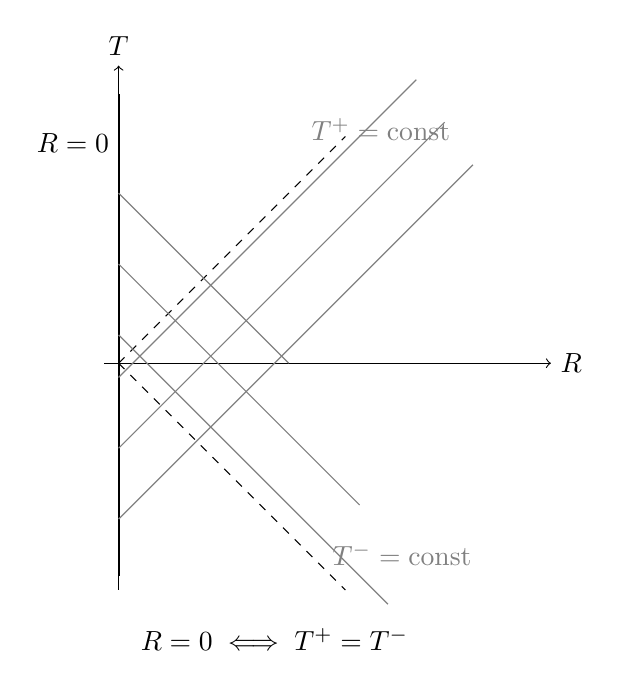
\begin{tikzpicture}[scale=0.9]
\draw[->] (-0.2,0) -- (6.1,0) node[right] {$R$};
\draw[->] (0,-3.2) -- (0,4.2) node[above] {$T$};

\draw[thick] (0,-3.0) -- (0,3.8);
\node[left] at (0,3.1) {$R=0$};

\draw[dashed] (0,0) -- (3.2,3.2);
\draw[dashed] (0,0) -- (3.2,-3.2);

\draw[gray] (0,2.4) -- (2.4,0);
\draw[gray] (0,1.4) -- (3.4,-2.0);
\draw[gray] (0,0.4) -- (3.8,-3.4);

\draw[gray] (0,-2.2) -- (5.0,2.8);
\draw[gray] (0,-1.2) -- (4.6,3.4);
\draw[gray] (0,-0.2) -- (4.2,4.0);

\node[gray] at (3.7,3.3) {$T^+=\mathrm{const}$};
\node[gray] at (4.0,-2.7) {$T^-=\mathrm{const}$};

\node at (2.2,-3.9) {$R=0 \iff T^+=T^-$};
\end{tikzpicture}
\caption{Vẽ lại rõ ràng mặt phẳng \(T\)-\(R\). Hai họ đường null là các đường mức của \(T^+\) và \(T^-\), còn đường \(R=0\) tương đương với \(T^+=T^-\).}
\end{figure}

Bây giờ ta compact hóa. Ta đưa vào hai tọa độ null mới \(U^\pm\), mỗi tọa độ thu được từ \(T^\pm\) tương ứng bằng cùng một hàm đơn điệu bị chặn \(F\):
\begin{align}
U^+ &= F(T^+), &
U^- &= F(T^-),
\end{align}
với
\begin{equation}
F(+\infty)=1,
\qquad
F(-\infty)=-1.
\end{equation}
Lựa chọn thuận tiện trong bài giảng là
\begin{equation}
F(x)=\tanh x,
\end{equation}
để rồi
\begin{equation}
U^+ = \tanh(T^+),
\qquad
U^- = \tanh(T^-).
\end{equation}
Không có gì đặc biệt về mặt nguyên tắc ở hàm tang hyperbol. Nó chỉ đơn giản là một hàm trơn với hành vi giới hạn thích hợp, và vì thế nó nén các miền tọa độ vô hạn xuống thành những miền hữu hạn.

Cấu trúc null được bảo toàn vì một lý do đơn giản. Nếu một tia sáng xuyên tâm đi vào có \(T^+=\text{const}\), thì
\[
U^+=F(T^+)=\text{const},
\]
và tương tự, nếu một tia sáng xuyên tâm đi ra có \(T^-=\text{const}\), thì
\[
U^-=F(T^-)=\text{const}.
\]
Do đó phép compact hóa tái tham số hóa riêng rẽ hai hướng null, và các tia sáng xuyên tâm vẫn là những đường \(45^\circ\). Đường gốc cũng được biến đổi theo một cách gọn gàng tương tự:
\[
T^+=T^- \Longrightarrow U^+=U^-.
\]

Đến đây, nửa mặt phẳng vô hạn của không-thời gian phẳng đã được nén thành một tam giác hữu hạn. Bài giảng tiếp đó chỉ cho ta cách đọc các biên của nó. Vô cùng không gian sụp lại thành một điểm duy nhất \(i^0\). Vô cùng kiểu thời gian trong tương lai và quá khứ là \(i^+\) và \(i^-\). Hai biên null là \(\mathcal{I}^+\) và \(\mathcal{I}^-\), thường được đọc là scri-plus và scri-minus, là nơi các tia sáng đi vào và đi ra có điểm đầu và điểm cuối.

\begin{figure}[htbp]
\centering
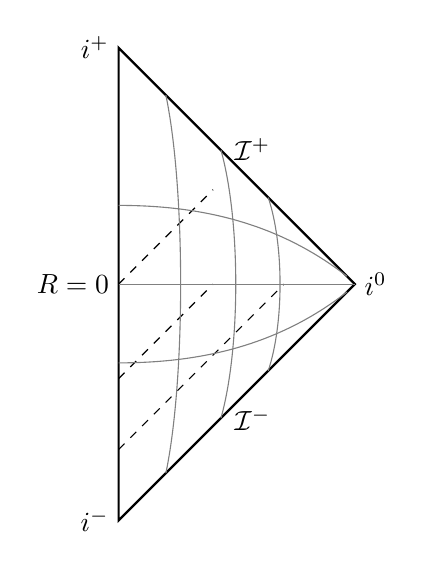
\begin{tikzpicture}[scale=1.0]
\draw[thick] (0,-3) -- (0,3) -- (3,0) -- cycle;

\node[left] at (0,3) {$i^+$};
\node[left] at (0,-3) {$i^-$};
\node[right] at (3,0) {$i^0$};
\node[left] at (0,0) {$R=0$};
\node[above right] at (1.35,1.45) {$\mathcal{I}^+$};
\node[below right] at (1.35,-1.45) {$\mathcal{I}^-$};

\draw[dashed] (0,-2.1) -- (2.1,0.0);
\draw[dashed] (0,-1.2) -- (1.2,0.0);
\draw[dashed] (0,0.0) -- (1.2,1.2);

\draw[gray] (0,0) -- (3,0);
\draw[gray] (0,1.0) .. controls (1.0,1.0) and (2.0,0.8) .. (2.9,0.1);
\draw[gray] (0,-1.0) .. controls (1.0,-1.0) and (2.0,-0.8) .. (2.9,-0.1);

\draw[gray] (0.6,-2.4) .. controls (0.85,-1.2) and (0.85,1.2) .. (0.6,2.4);
\draw[gray] (1.3,-1.7) .. controls (1.55,-0.8) and (1.55,0.8) .. (1.3,1.7);
\draw[gray] (1.9,-1.1) .. controls (2.1,-0.5) and (2.1,0.5) .. (1.9,1.1);
\end{tikzpicture}
\caption{Giản đồ Penrose cho không-thời gian phẳng sau khi rút gọn theo bán kính. Các đường thời gian không đổi chạy ra ngoài về phía \(i^0\), còn các đường bán kính không đổi đi lên từ \(i^-\) đến \(i^+\).}
\end{figure}

Cần ghi nhớ thêm một điểm cuối cùng từ bài giảng. Những giản đồ này \emph{không} bảo toàn độ lớn theo metric. Chúng bảo toàn cấu trúc nhân quả. Đó là bất biến mà ta nhắm tới.

\begin{classroomqa}
\audiencequestion{Các đường thời gian không đổi sau khi compact hóa có phải là thẳng không?}
\lecturerresponse{Đối với ánh xạ đã chọn, chỉ lát cắt đối xứng \(T=0\) là thẳng. Các đường \(T\) không đổi khác thì cong, và hình dạng chi tiết của chúng phụ thuộc vào hàm compact hóa. Các lát cắt rất muộn dồn ngày càng sát biên trên hơn, mặc dù thời gian thông thường vẫn tiếp tục không bị chặn trên.
\lecturetimestamp{00:29:11--00:30:12}}
\end{classroomqa}

\section{Hình học Schwarzschild compact hóa}

Dựa trên phép dựng trong không gian phẳng, giờ ta quay lại lỗ đen và làm lại điều tương tự. Ta compact hóa hình học Kruskal bằng cách đưa vào các tọa độ null và ép các khoảng vô hạn vào một hình hữu hạn. Giảng viên mô tả kết quả như một bức tranh nhân quả dạng hình chữ nhật nghiêng hoặc giống hình thoi: chân trời xuất hiện như một biên null, các đường thế giới lơ lửng ở miền ngoài vẫn nằm ngoài nó, và miền bên trong kết thúc trên một kỳ dị nay đã hiện ra trên trang.

Điểm vật lý then chốt là, trong trải nghiệm của quan sát viên rơi vào, kỳ dị \emph{không} nằm ở vô cực. Một khi đã vượt qua chân trời, phần thời gian riêng còn lại trước khi đâm vào kỳ dị là hữu hạn. Giản đồ Penrose làm cho điều này trở nên hiển nhiên về mặt trực quan.

Chân trời lại một lần nữa được xác định bởi điều kiện Schwarzschild
\begin{equation}
1-\frac{2MG}{r}=0
\qquad \Longleftrightarrow \qquad
r=2MG.
\end{equation}
Đẳng thức \(r=2MG\) đánh dấu bán kính tại đó thừa số Schwarzschild đổi dấu.

\begin{figure}[htbp]
\centering
\includegraphics[width=0.72\textwidth]{lecture_08_figure_04.png}
\caption{Phác thảo trên bảng đối chiếu bức tranh mở rộng hình thức với miền lỗ đen có ý nghĩa vật lý. Nhãn đỏ \emph{kỳ dị} được ghi tường minh trên bảng.}
\lectureframe{00:37:59}
\end{figure}

\begin{figure}[htbp]
\centering
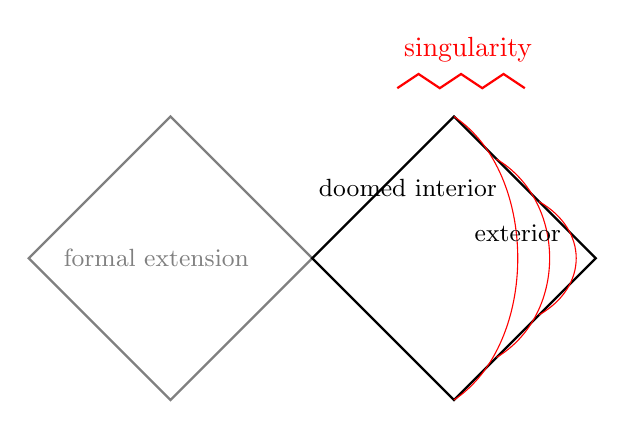
\begin{tikzpicture}[scale=0.9]
\draw[gray,thick] (-4,0) -- (-2,2) -- (0,0) -- (-2,-2) -- cycle;
\draw[thick] (0,0) -- (2,2) -- (4,0) -- (2,-2) -- cycle;

\draw[red,thick] (1.2,2.4) -- (1.5,2.6) -- (1.8,2.4) -- (2.1,2.6) -- (2.4,2.4) -- (2.7,2.6) -- (3.0,2.4);
\node[red] at (2.2,2.95) {singularity};

\draw[red] (2.0,-2.0) .. controls (3.2,-1.2) and (3.2,1.2) .. (2.0,2.0);
\draw[red] (2.6,-1.4) .. controls (3.6,-0.8) and (3.6,0.8) .. (2.6,1.4);
\draw[red] (3.2,-0.8) .. controls (3.9,-0.4) and (3.9,0.4) .. (3.2,0.8);

\node at (2.9,0.35) {\small exterior};
\node at (1.35,1.0) {\small doomed interior};
\node[gray] at (-2.2,0.0) {\small formal extension};
\end{tikzpicture}
\caption{Một bản vẽ lại thận trọng của bức tranh nhân quả được nhấn mạnh trong bài giảng: miền ngoài còn tồn tại, miền trong tất phải diệt vong, kỳ dị tương lai, và sự tương phản với phần hình thức bổ sung của phép mở rộng.}
\end{figure}

Ở đây bài giảng nói rất trực tiếp. Nếu ta ở miền ngoài, ta vẫn có thể thoát ra, hoặc có thể rơi vào. Nếu ta ở miền trong, ta đã bị định sẵn diệt vong. Giản đồ này đã nói lên mọi điều quan trọng về chuyển động nhân quả hướng tương lai.

Các góc phần tư \(III\) và \(IV\) là những phần hợp lệ của nghiệm Kruskal mở rộng tối đa. Miền \(III\) cho một miền ngoài thứ hai, và miền \(IV\) là miền lỗ đen đảo chiều thời gian. Tuy nhiên, chúng không xuất hiện trong không-thời gian của một lỗ đen thông thường được tạo ra bởi sự sụp đổ. Nghiệm mở rộng đặc biệt có tính chỉ dẫn về mặt toán học chính vì phép dựng suy sụp sẽ cho ta thấy những phần nào phải bị loại bỏ.

\section{Các lát cắt không gian, các mặt cầu 2 chiều, và cầu Einstein--Rosen}

Bây giờ hãy cố định giản đồ compact hóa tại một lát cắt kiểu không gian và hỏi lát cắt đó trông như thế nào khi được xem là \emph{không gian} chứ không phải không-thời gian. Đây là chỗ hình ảnh lỗ sâu xuất hiện, và cũng là chỗ không được để bức tranh không gian đi xa hơn lập luận nhân quả.

Vì các phương góc đã bị lược bỏ, mỗi điểm của giản đồ xuyên tâm biểu diễn một mặt cầu 2 chiều. Với bán kính Schwarzschild \(r\), diện tích của mặt cầu đó là
\begin{equation}
A=4\pi r^2.
\end{equation}
Vì thế, một lát cắt kiểu không gian là một họ các mặt cầu 2 chiều, chứ không chỉ đơn thuần là một đường một chiều. Kích thước của chúng thay đổi khi ta di chuyển dọc theo lát cắt ấy.

Ở rất xa, các mặt cầu này rất lớn. Khi đi vào trong, bán kính của chúng co lại cho đến khi đạt giá trị nhỏ nhất tại chân trời,
\begin{equation}
r_{\min}=2MG.
\end{equation}
Nếu tiếp tục đi qua phần mở rộng hình thức, các mặt cầu lại nở ra về phía một miền tiệm cận khác. Đây là bức tranh cầu Einstein--Rosen.

\begin{figure}[htbp]
\centering
\includegraphics[width=0.72\textwidth]{lecture_08_figure_05.png}
\caption{Giản đồ Kruskal mở rộng với lát cắt kiểu không gian màu xanh lục được dùng để dựng hình học của cầu. Mỗi điểm trên lát cắt ấy biểu diễn một mặt cầu 2 chiều; bán kính nhỏ nhất được đánh dấu là \(r=2MG\).}
\lectureframe{00:41:30}
\end{figure}

Trên bảng chỉ viết ra một phần của thừa số Schwarzschild liên quan,
\begin{equation}
1-\frac{2MG}{r},
\end{equation}
và cổ họng xuất hiện tại chính bán kính đặc biệt ấy, \(r=2MG\).

\begin{figure}[htbp]
\centering
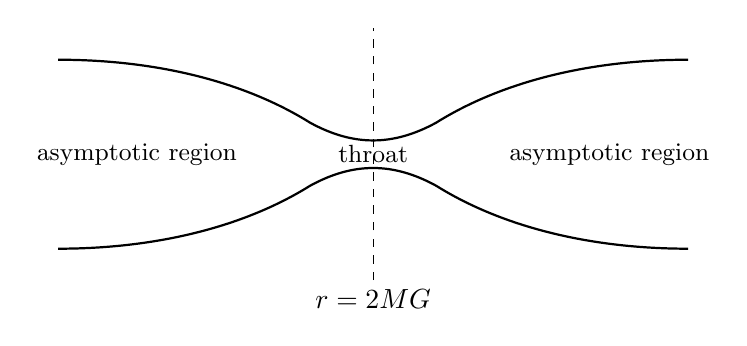
\begin{tikzpicture}[scale=1.0]
\draw[thick] (-4,1.2)
.. controls (-2.7,1.2) and (-1.6,0.9) .. (-0.8,0.4)
.. controls (-0.25,0.1) and (0.25,0.1) .. (0.8,0.4)
.. controls (1.6,0.9) and (2.7,1.2) .. (4,1.2);

\draw[thick] (-4,-1.2)
.. controls (-2.7,-1.2) and (-1.6,-0.9) .. (-0.8,-0.4)
.. controls (-0.25,-0.1) and (0.25,-0.1) .. (0.8,-0.4)
.. controls (1.6,-0.9) and (2.7,-1.2) .. (4,-1.2);

\draw[dashed] (0,-1.6) -- (0,1.6);
\node[below] at (0,-1.6) {$r=2MG$};
\node at (0,0) {\small throat};
\node at (-3.0,0) {\small asymptotic region};
\node at (3.0,0) {\small asymptotic region};
\end{tikzpicture}
\caption{Lát cắt không gian sơ lược qua hình học Schwarzschild mở rộng. Đây là một phục dựng thận trọng của bức tranh cây cầu trong bài giảng, không phải một phép tính nhúng theo nghĩa đen.}
\end{figure}

Bây giờ đến phần hiệu chỉnh. Lát cắt gợi ra một cây cầu giữa hai miền tiệm cận, nên nó dễ làm nảy sinh ý nghĩ rằng ta có thể đi từ vũ trụ này sang vũ trụ kia bằng cách băng qua cổ hẹp. Bài giảng trước hết để cho gợi ý đó xuất hiện, rồi bác bỏ nó bằng lập luận nhân quả. Để đi từ một miền ngoài sang miền ngoài kia, một đường thế giới sẽ phải trở nên ít dốc hơn một đường null \(45^\circ\) ở đâu đó trên giản đồ Penrose. Điều đó bị cấm. Vì vậy, cầu Einstein--Rosen là không thể đi xuyên qua.

Giảng viên cũng nhấn mạnh vì sao bức tranh không gian có thể gây hiểu lầm. Nó là bức tranh của \emph{không gian tại một thời điểm}; nhưng đơn giản là không có đủ thời gian nhân quả để đi xuyên qua. Nói một cách lỏng lẻo, cây cầu mở ra rồi khép lại trước khi bất cứ thứ gì có thể vượt qua nó. Tốt hơn nữa, ta chỉ cần nhìn lại giản đồ Penrose và đọc ra câu trả lời nhân quả.

\section{Dựng một lỗ đen thực từ một vỏ null rơi vào}

Đến đây, bài giảng chuyển hẳn sang một bài toán khác. Ta không còn chỉ đọc ra các tính chất của một lỗ đen vĩnh cửu nữa. Ta đang dựng một lỗ đen thực.

Mô hình được chọn vì tính đơn giản. Ta hình dung không phải một ngôi sao đang sụp đổ với cấu trúc bên trong rối rắm, mà là một vỏ cầu mỏng gồm bức xạ đi vào. Đó là một vỏ ánh sáng, và do đó chuyển động vào trong với tốc độ ánh sáng. Ở bán kính đủ nhỏ, năng lượng trên vỏ ấy tập trung đủ chặt để một lỗ đen hình thành.

Yếu tố thứ hai là định lý vỏ trong dạng của thuyết tương đối rộng.

\paragraph{Nhận xét.} Đối với vỏ đối xứng cầu được dùng trong bài giảng này, miền bên trong là không-thời gian phẳng, còn miền bên ngoài là Schwarzschild. Đây là định lý vỏ theo nghĩa thao tác, hay một mệnh đề kiểu Birkhoff, được dùng trong bài giảng. Ở đây không chứng minh điều đó.

Giảng viên dẫn nhập điều này bằng cách trước hết nhắc lại định lý vỏ Newton: bên trong một vỏ cầu không có trường hấp dẫn, còn bên ngoài vỏ thì trường giống hệt trường của một khối điểm đặt tại tâm. Sau đó ông phát biểu phiên bản tương đối tính tương ứng dưới dạng duy nhất cần ở đây: bên trong là phẳng, bên ngoài là Schwarzschild. Vỏ có thể chuyển động; quy tắc vẫn vậy.

Như thế là đủ để dựng không-thời gian suy sụp. Bản thân vỏ là null, nên nó phải được vẽ ở góc \(45^\circ\). Ở một phía của đường null đó, hình học là phẳng. Ở phía kia, nó là Schwarzschild. Ta có thể tóm tắt quy tắc thành
\begin{equation}
\begin{aligned}
\text{inside shell} &= \text{flat spacetime},\\
\text{outside shell} &= \text{Schwarzschild geometry}.
\end{aligned}
\end{equation}

Khi đó, quy tắc ghép trở nên gần như đơn giản đến mức đáng ngượng:

\begin{enumerate}
\item Vẽ giản đồ Penrose phẳng và chỉ giữ lại miền nằm phía trong vỏ đi vào.
\item Vẽ giản đồ Penrose Schwarzschild và chỉ giữ lại miền nằm phía ngoài chính vỏ đó.
\item Vứt bỏ những phần sai.
\item Khâu hai phần còn lại với nhau dọc theo quỹ đạo của vỏ.
\end{enumerate}

Đây chính xác là cách bài giảng triển khai trên bảng: bỏ đi nửa sai của một hình, bỏ đi nửa sai của hình kia, rồi ghép hai nửa đúng lại với nhau dọc theo vỏ.

\begin{figure}[htbp]
\centering
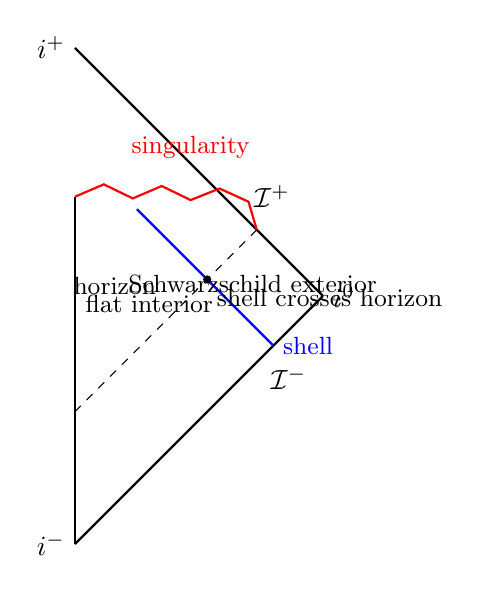
\begin{tikzpicture}[scale=1.05]
\coordinate (im) at (0,-3.0);
\coordinate (ip) at (0,3.0);
\coordinate (i0) at (3.0,0.0);
\coordinate (S)  at (0,1.2);
\coordinate (E)  at (2.2,0.8);
\coordinate (P)  at (2.4,-0.6);
\coordinate (Q)  at (0.75,1.05);
\coordinate (H)  at (0,-1.4);
\coordinate (X)  at (1.6,0.2);

\draw[thick] (im) -- (S);
\draw[thick] (im) -- (i0);
\draw[thick] (ip) -- (i0);

\draw[red,thick] (S) -- (0.35,1.35) -- (0.7,1.18) -- (1.05,1.33) -- (1.4,1.16) -- (1.75,1.30) -- (2.1,1.14) -- (E);
\node[red,above] at (1.4,1.55) {\small singularity};

\draw[thick,blue] (P) -- (Q);
\node[blue,right] at (P) {\small shell};

\draw[dashed] (H) -- (E);
\node[above left] at (1.1,-0.1) {\small horizon};

\filldraw (X) circle (1.2pt);
\node[below right] at (X) {\small shell crosses horizon};

\node at (0.9,-0.1) {\small flat interior};
\node at (2.15,0.15) {\small Schwarzschild exterior};

\node[left] at (im) {$i^-$};
\node[left] at (ip) {$i^+$};
\node[right] at (i0) {$i^0$};
\node[below right] at (2.25,-0.75) {$\mathcal{I}^-$};
\node[above right] at (2.05,0.95) {$\mathcal{I}^+$};
\end{tikzpicture}
\caption{Phục dựng nhân quả của hình học suy sụp. Vỏ là một đường null đi vào; không-thời gian phẳng được giữ ở phía trong của nó và hình học Schwarzschild được giữ ở phía ngoài của nó.}
\end{figure}

\begin{figure}[htbp]
\centering
\includegraphics[width=0.76\textwidth]{lecture_08_figure_06.png}
\caption{Cấu dựng hoàn chỉnh trên bảng sau khi phần trong phẳng và phần ngoài Schwarzschild đã được ghép dọc theo vỏ rơi vào màu xanh. Đường đứt nét \(45^\circ\) đang được lần ngược trở lại từ điểm cuối tương lai của kỳ dị để xác định chân trời sự kiện.}
\lectureframe{00:57:30}
\end{figure}

Bản thân vỏ không trải qua điều gì đặc biệt tại thời điểm nó chỉ đơn thuần đi qua từ phần phẳng của giản đồ sang phần Schwarzschild. Nó là một vỏ kiểu ánh sáng, và tiếp tục đi vào cho đến khi chạm kỳ dị. Cấu trúc cốt yếu không nằm ở bất kỳ kịch tính cục bộ nào trên vỏ; nó nằm ở tổ chức nhân quả của không-thời gian đã được ghép.

\begin{classroomqa}
\audiencequestion{Có một sự gián đoạn nào không khi vỏ suy sụp đi qua bán kính Schwarzschild của nó?}
\lecturerresponse{Không. Không có gì kỳ dị cục bộ xảy ra tại lần băng qua đó.
Vỏ tiếp tục trên quỹ đạo null của nó. Sự kiện đặc biệt là về mặt nhân quả:
sau khi vỏ đã vượt qua bán kính \(2MG\) của chính nó, không một đường đi hướng tương lai nào
có thể đưa nó trở lại vô cực.
\lecturetimestamp{00:56:19--00:56:42}}
\end{classroomqa}

\section{Chân trời trước khi đến nơi: câu đố về chân trời sự kiện}

Giờ là đỉnh điểm về mặt khái niệm của bài giảng. Khi đã dựng xong không-thời gian sụp đổ, câu hỏi tự nhiên là: chân trời ở đâu? Hay như giảng viên nói, điểm không thể quay lại ở đâu?

\paragraph{Định nghĩa.} Chân trời sự kiện là ranh giới giữa những biến cố mà từ đó vẫn còn có thể gửi một tín hiệu nhân quả hướng tương lai tới \(\mathcal{I}^+\) và những biến cố mà từ đó không thể làm vậy.

Bài giảng xác định nó trên giản đồ. Hãy bắt đầu từ góc nơi kỳ dị gặp vô cực null tương lai, rồi truy vết ngược một đường null \(45^\circ\). Đường null được truy vết ngược đó chính là chân trời sự kiện.

Nhưng rồi giảng viên nhấn mạnh một điểm thứ hai, và chính điểm này làm sinh viên bối rối. Chân trời không phải chỉ đơn giản xuất hiện đúng vào lúc lớp vỏ đi qua bán kính Schwarzschild của chính nó rồi sau đó giữ nguyên ở đó. Trong hình vẽ phóng to trên bảng, chân trời bắt đầu như một vùng bị bẫy rất nhỏ gần tâm, mở rộng ra ngoài qua một phần của không-thời gian vẫn còn phẳng, và chỉ về sau mới gặp lớp vỏ đang đi vào. Tại biến cố gặp nhau đó, lớp vỏ đi qua bán kính Schwarzschild của chính nó. Phía trên biến cố ấy, chân trời là chân trời thông thường có bán kính không đổi của lỗ đen đã hình thành hoàn chỉnh.

\begin{figure}[htbp]
\centering
\resizebox{0.96\linewidth}{!}{%
\begin{tikzpicture}[scale=1.08,>=Latex]
\coordinate (im) at (0,-3.0);
\coordinate (ip) at (0,3.0);
\coordinate (i0) at (3.0,0.0);
\coordinate (S)  at (0,1.2);
\coordinate (E)  at (2.2,0.8);
\coordinate (P)  at (2.4,-0.6);
\coordinate (Q)  at (0.75,1.05);
\coordinate (H)  at (0,-1.4);
\coordinate (X)  at (1.6,0.2);

\draw[thick] (im) -- (S);
\draw[thick] (im) -- (i0);
\draw[thick] (ip) -- (i0);

\draw[red,thick] (S) -- (0.35,1.35) -- (0.7,1.18) -- (1.05,1.33) -- (1.4,1.16) -- (1.75,1.30) -- (2.1,1.14) -- (E);
\node[red,above left] at (S) {\small singularity};

\draw[very thick,red] (H) -- (E);

\draw[thick,blue] (P) -- (Q);

\filldraw (X) circle (1.2pt);

\draw[gray] (0.0,-2.1) .. controls (0.85,-1.95) and (1.9,-1.3) .. (2.8,-0.2);
\draw[gray] (0.0,-1.2) .. controls (0.95,-1.0) and (1.8,-0.45) .. (2.45,0.35);
\draw[gray] (0.0,-0.2) .. controls (0.8,-0.05) and (1.45,0.35) .. (1.95,0.95);

\node[below right] at (2.28,-0.72) {$\mathcal{I}^-$};
\node[above right] at (2.12,0.92) {$\mathcal{I}^+$};

\draw[very thick,red] (3.2,-1.15) -- (3.75,-1.15);
\node[anchor=west] at (3.85,-1.15) {\small event horizon};
\draw[thick,blue] (3.2,-1.55) -- (3.75,-1.55);
\node[anchor=west] at (3.85,-1.55) {\small infalling shell};
\filldraw (3.48,-1.95) circle (1.2pt);
\node[anchor=west] at (3.85,-1.95)
  {\small shell reaches \(r=2MG\)};
\end{tikzpicture}
}
\caption{Giản đồ sụp đổ với chân trời sự kiện được truy vết ngược được nhấn mạnh. Một phần của chân trời nằm trong một vùng vẫn còn phẳng cục bộ và vỏ vẫn chưa tới đó.}
\end{figure}

Đây là hiệu ứng nổi bật mà phần còn lại của bài giảng tập trung vào. Một phần của chân trời nằm trong không-thời gian phẳng. Vỏ vẫn chưa tới đó, và nó thậm chí còn chưa hiện trên nón ánh sáng quá khứ của người quan sát. Người quan sát không cảm thấy trường hấp dẫn nào mà vẫn không thể thoát ra. Lý do không phải là một lực cục bộ. Đó là tương lai nhân quả toàn cục của biến cố ấy.

\begin{classroomqa}
\audiencequestion{Cách dựng này nói rằng người ta không thể đi qua vỏ, hay rằng người ta không thể đi qua chân trời? Vào lúc chân trời của nó vẫn còn nằm bên trong vỏ, thì vỏ ở đâu?}
\lecturerresponse{Có thể đi qua vỏ. Chân trời là một mặt null khác: đó là ranh giới giữa những biến cố có thể liên lạc với \(\mathcal I^+\) và những biến cố không thể. Vỏ đi vào gặp ranh giới đó đúng vào lúc nó đi qua bán kính Schwarzschild gắn với tổng năng lượng của nó. Trước khi gặp nhau, một phần của chân trời sự kiện đi qua phần bên trong phẳng; sau khi gặp nhau, vỏ nằm bên trong hố đen đã hình thành xong.
\lecturetimestamp{00:58:42--01:01:06}}
\end{classroomqa}

\begin{classroomqa}
\audiencequestion{Nếu phần bên trong là phẳng và vỏ vẫn còn ở xa, thì tại sao một người ở ngay bên trong chân trời lại không thể đi bộ băng qua nó trước khi vỏ tới?}
\lecturerresponse{Hãy vẽ đường thế giới hướng ra ngoài nhanh nhất có thể, một tia sáng \(45^\circ\). Từ một biến cố nằm bên trong chân trời được truy vết ngược, ngay cả tia đó cũng gặp vỏ đi vào quá muộn và kết thúc tại kỳ dị. Đi bộ còn chậm hơn nữa. Cụm từ \emph{vỏ vẫn chưa đi qua} là chưa đầy đủ chừng nào chưa chọn một tọa độ thời gian; giản đồ nhân quả cung cấp câu trả lời độc lập với tọa độ. Bức xạ nền vi sóng vũ trụ đi tới không phải là một ví dụ tương tự, vì nó không phải là một vỏ cầu sụp vào tạo ra hình học này.
\lecturetimestamp{01:01:07--01:04:03}}
\end{classroomqa}

\section{Gương và những nỗ lực thay đổi tương lai}

Giờ đây các câu hỏi biến giản đồ thành một phòng thí nghiệm. Giả sử một vỏ ánh sáng đi vào có thể bị phản xạ trước khi nó bị bẫy. Khi đó lịch sử sụp đổ được giả định sẽ thay đổi, và chân trời sự kiện cũng thay đổi theo. Đây không phải là mâu thuẫn: chân trời sự kiện chỉ được xác định sau khi toàn bộ lịch sử không-thời gian đã được chỉ rõ.

\begin{classroomqa}
\audiencequestion{Điều gì xảy ra nếu đặt một chiếc gương phản xạ hoàn hảo ngay bên ngoài bán kính Schwarzschild giả định để vỏ nảy bật trở ra?}
\lecturerresponse{Trong lịch sử lý tưởng hóa ấy, đường null đi vào quay ra ngoài tại chiếc gương và đi tới biên tương lai; hố đen trong giản đồ ban đầu không hình thành. Một chiếc gương thực sự không trọng lượng là không thể có, và một chiếc gương vật lý mang thêm năng lượng-ứng suất của riêng nó, nhưng thí nghiệm tưởng tượng làm rõ điểm logic này: chỉ sau khi vỏ đi qua chân trời sự kiện thực sự thì việc thoát ra mới không còn có thể.
\lecturetimestamp{01:04:33--01:05:54}}
\end{classroomqa}

\begin{classroomqa}
\audiencequestion{Liệu một người quan sát biết vỏ sắp tới có thể mau chóng gửi ra một chiếc gương hay một tín hiệu để làm nó quay đầu không?}
\lecturerresponse{Chỉ khi thiết bị cần thiết có thể được đặt bên ngoài chân trời đủ sớm. Alice có thể thu xếp trước để Bob gửi vỏ, và vì thế có thể biết điều sắp đến trước khi cô nhìn thấy nó. Tuy nhiên, một khi biến cố của cô đã ở bên trong chân trời, thì cả một chiếc gương lẫn một chỉ thị đều không thể tới điểm bên ngoài cần thiết kịp thời. Việc biết trước thí nghiệm tương lai không mở ra một đường nhân quả mà giản đồ cấm.
\lecturetimestamp{01:05:55--01:08:18}}
\end{classroomqa}

\begin{classroomqa}
\audiencequestion{Điều gì xảy ra với một chiếc gương đã ở sẵn bên trong chân trời, và kỳ dị có ở xa vô hạn trong tương lai của nó hay không?}
\lecturerresponse{Chiếc gương đơn giản chỉ là thêm một vật tất phải diệt vong. Nó có thể phản xạ ánh sáng tại chỗ, nhưng ánh sáng đã phản xạ, chiếc gương và Alice đều kết thúc tại kỳ dị. Một đường thế giới rơi vào điển hình chạm tới đó trong thời gian riêng hữu hạn. Chỉ góc trên lý tưởng của giản đồ compact hóa là ở xa vô hạn. Cố gắng ở lại gần góc đó sẽ đòi hỏi gia tốc và năng lượng không bị chặn trên; hơn nữa, giữa các biến cố cố định, một đồng hồ gia tốc tích lũy ít thời gian riêng hơn một đồng hồ quán tính, chứ không nhiều hơn.
\lecturetimestamp{01:08:19--01:10:19}}
\end{classroomqa}

\begin{classroomqa}
\audiencequestion{Nếu vỏ đang sụp vào là khổng lồ, thì một người ở bên trong vỏ nhưng xa tâm cuối cùng của nó có thể đơn giản ở yên đó khi nó đi qua hay không?}
\lecturerresponse{Có, miễn là biến cố của người đó vẫn còn ở ngoài chân trời sự kiện. Ở bên trong vỏ vật chất không đồng nghĩa với ở bên trong hố đen. Bức xạ có thể đánh trúng và làm tổn hại người quan sát, nhưng đó là một tương tác cục bộ với vỏ và tách biệt với câu hỏi nhân quả về việc thoát ra.
\lecturetimestamp{01:10:21--01:11:24}}
\end{classroomqa}

\section{Các lát cắt thời gian và chân trời đang mở rộng}

Một \emph{thời điểm} trong không-thời gian cong có nghĩa là một siêu mặt kiểu không gian được chọn. Một họ các mặt như vậy tạo thành một phân lá, và việc gán một số cho mỗi mặt xác định một tọa độ thời gian. Các phân lá khác nhau cắt cùng một giản đồ sụp đổ theo những cách khác nhau. Chúng không thống nhất về việc những biến cố xa nào là đồng thời, nhưng chúng không làm thay đổi những tia null nào đi tới vô cực.

\begin{figure}[htbp]
\centering
\includegraphics[width=0.77\textwidth]{lecture_08_figure_07.png}
\caption{Giản đồ trên bảng ở giai đoạn sau với một số lát cắt kiểu không gian màu xanh lục. Các lát cắt cung cấp một tọa độ thời gian; các biên null màu đen và các quan hệ nhân quả của chúng không phụ thuộc vào lựa chọn đó.}
\lectureframe{01:17:30}
\end{figure}

\begin{classroomqa}
\audiencequestion{Có thể phát biểu lại câu đố bằng cách so sánh, tại một thời điểm, khoảng cách từ người quan sát đến chân trời với khoảng cách từ chân trời đến vỏ hay không?}
\lecturerresponse{Điều đó có thể là một trực giác hữu ích sau khi đã chọn một phân lá, nhưng cụm từ \emph{tại một thời điểm} phụ thuộc vào tọa độ. Cách dựng rõ ràng nhất là vẽ một họ các lát cắt kiểu không gian. Các lát sớm cắt qua một vỏ lớn và không có vùng bị bẫy trung tâm nào; các lát muộn cắt qua chân trời đang mở rộng bên trong vỏ vẫn còn đang rơi vào; một lát đặc biệt đi qua biến cố nơi vỏ đi qua bán kính Schwarzschild của chính nó.
\lecturetimestamp{01:11:26--01:14:21}}
\end{classroomqa}

\begin{classroomqa}
\audiencequestion{Bán kính Schwarzschild có tăng lên khi chân trời mở ra phía ngoài không, và vì sao chân trời vẫn tiếp tục lớn lên sau khi vỏ đi qua nó?}
\lecturerresponse{Bán kính Schwarzschild cuối cùng \(2MG\) là cố định vì tổng khối lượng \(M\) là cố định. Thứ tăng lên trên các lát cắt kiểu không gian ban đầu là bán kính diện tích của tiết diện chân trời. Nó bắt đầu ở tâm, tăng lên cho đến khi gặp vỏ tại \(r=2MG\), rồi dừng lại. Phía trên biến cố gặp nhau, chân trời là đường \(r=2MG\) với \(r\) không đổi, mặc dù phép compact hóa không làm cho đường đó trông thẳng đứng hay đồng đều về metric.
\lecturetimestamp{01:14:22--01:16:15}}
\end{classroomqa}

\begin{classroomqa}
\audiencequestion{Điều gì xảy ra với một người quan sát ban đầu ở bán kính bằng một nửa bán kính Schwarzschild cuối cùng? Chẳng phải người quan sát ấy chỉ nên cảm thấy hấp dẫn khi vỏ tới hay sao?}
\lecturerresponse{Chính xác. Người quan sát trước hết đi qua chân trời sự kiện đang mở rộng khi vẫn còn ở trong không-thời gian phẳng và không cảm thấy lực đột ngột nào. Vỏ bức xạ đang rơi vào là một thực thể vật lý và về sau có thể được cảm nhận; chân trời sự kiện thì không. Việc đi qua nó chỉ có nghĩa là mọi đường nhân quả hướng tương lai giờ đây đều không tới được vô cực. Theo nghĩa chính xác đó, chân trời có tính chất như bóng ma.
\lecturetimestamp{01:16:17--01:17:45}}
\end{classroomqa}

\begin{classroomqa}
\audiencequestion{Liệu một quan sát viên khởi hành đủ sớm có thể chuyển động ra ngoài nhanh hơn chân trời đang mở rộng và thoát ra được không?}
\lecturerresponse{Có. Các sự kiện ở bên ngoài chân trời có các đường nhân quả đi ra ngoài tới \(\mathcal I^+\); các sự kiện ở bên trong thì không. Trên một lát cắt đã chọn, ta có thể so sánh khoảng cách theo phương bán kính còn lại với quãng thời gian trước khi lớp vỏ đang đi vào bịt kín lối thoát, nhưng các đường null mới cho phép kiểm tra chính xác. Không có quan sát viên nào thấy một chân trời vật chất đang lao ra ngoài, vì không có bề mặt cục bộ nào để quan sát.
\lecturetimestamp{01:17:46--01:18:54}}
\end{classroomqa}

\section{Những gì sơ đồ bảo toàn}

Các hình trên trang không được hiểu như một bản vẽ đúng tỷ lệ. Một góc nhỏ có thể biểu diễn một miền không-thời gian vô hạn, trong khi một mảng lớn có thể biểu diễn một khoảng vật lý khá nhỏ. Phép compact hóa cố ý hy sinh độ lớn theo metric để bảo toàn các hướng null. Điều còn lại là quan hệ nhân quả: ai có thể gửi tín hiệu cho ai, sự kiện nào có thể ảnh hưởng tới những sự kiện nào khác, và những đường thế giới nào bị mắc kẹt bởi giới hạn tốc độ ánh sáng.

\begin{classroomqa}
\audiencequestion{Nếu hình này làm méo các độ dài và thời gian nghiêm trọng đến vậy, thì nó biểu diễn điều gì một cách trung thực?}
\lecturerresponse{Nó biểu diễn các tia sáng và do đó là cấu trúc nhân quả. Để xác định chân trời sự kiện, hãy lần ngược tia null đi ra ngoài cuối cùng từ vô cực tương lai. Cố suy ra đáp án từ các khoảng cách biểu kiến trên trang là không đáng tin cậy. Một khi giản đồ nhân quả đã được vẽ, các câu hỏi về tín hiệu, việc thoát ra và sự không thể quay lại đều có câu trả lời hình học, mặc dù thang đo metric đã bị lược bỏ.
\lecturetimestamp{01:18:56--01:21:45}}
\end{classroomqa}

\begin{classroomqa}
\audiencequestion{Cần bao lâu để đủ quen thuộc với các giản đồ Penrose đến mức có thể dùng chúng một cách trực giác?}
\lecturerresponse{Không lâu. Chỉ dẫn thực hành là vẽ chúng, lần theo các đường null, và kiểm tra các đường thế giới khả dĩ cho đến khi các ràng buộc nhân quả trở nên quen thuộc. Trực giác ở đây có được nhờ làm việc với các giản đồ, chứ không phải nhờ phỏng đoán khi không dùng đến chúng.
\lecturetimestamp{01:21:49--01:22:05}}
\end{classroomqa}

\begin{classroomqa}
\audiencequestion{Phương pháp trực quan này có phải là điều ngược lại với cơ học lượng tử, nơi toán học thường đáng tin hơn một hình ảnh không?}
\lecturerresponse{Ở mức độ đáng kể, đúng vậy. Thuyết tương đối rộng là vật lý cổ điển. Không-thời gian cong bốn chiều khó mà hình dung theo nghĩa đen, và một giản đồ Penrose vẫn còn trừu tượng, nhưng hình học nhân quả của nó có thể được vẽ ra và khảo sát xa hơn nhiều so với mức mà thực tại nền tảng của cơ học lượng tử cho phép. Chính sự khác biệt đó là một phần khiến các giản đồ này mạnh mẽ đến vậy.
\lecturetimestamp{01:22:05--01:22:58}}
\end{classroomqa}